%  TEX root = ../main.tex
% lezione 2 - 01/10/2021
\chapter{Problemi di ottimizzazione}
\section {Introduzione}
Un problema di \textbf{ottimizzazione} è caratterizzato da: 
\begin{enumerate}
  \item l'insieme degli input $I_{\Pi}$;
  \item l'insieme degli output $O_{\Pi}$;
  \item  una funzione che ad ogni input associa una famiglia di output:
    $Amm_{\Pi} : I_{\Pi} \rightarrow (2^{O_{\Pi}} \setminus \emptyset)$;
  \item il tipo del problema $Tipo_{\Pi} \in \{Min, Max\}$; e
  \item una funzione da una coppia input-output ai naturali
    $$
	c_{\Pi}: I_{\Pi} \times O_{\Pi} \rightarrow \mathbb{N}
    $$
    che formalizza il concetto di \textbf{costo} di una soluzione - per un problema 
    di minizzazione, l'obiettivo sarà scegliere l'output con costo minore. 

\end{enumerate}
Le proprietà $3$, $4$ e $5$ formalizzano ulteriormente l'insieme $Sol_{\Pi}$ definito in precedenza. 
\subsection{Esempi}
\subsubsection{MaxSat}

\popt{MaxSAT}
{CNF ben formate}
{$\mathbb{N}$} 
{Qual è il numero massimo di clausole che si possono verificare?} 
{Assegnamenti di valori di verità coerenti} 
{$Max$}
{Numero di clausole rese vere}

\noindent
Le istanze di questo problema sono formule ben formate in forma normale congiunta
(ossia CNF); le soluzioni ammissibili sono assegnamenti di valori di verità; il
costo (o \textit{funzione obiettivo}) è il numero di clausole rese vere.
\textsc{MaxSat} ha chiaramente $Tipo_{\Pi} = Max$, in quanto l'obiettivo è
massimizzare il numero di clausole verificate.

In alcuni frangenti potrebbe causarsi una certa ambiguità: l'algoritmo cerca
\textit{il valore} della soluzione ottimale o \textit{la soluzione} ottimale
stessa? Nel nostro corso diciamo che cerchiamo la soluzione stessa, in quanto il
suo valore è calcolabile con la funzione di costo, e la indicheremo con la
notazione $y^*(x)$; inoltre, indicheremo il costo della soluzione ottimale con
$c^*(x) = c_{\pi}(y^*(x))$

\section{Rapporto di prestazioni}
Dato un input $x \in I_{\Pi}$ e $y \in Amm_{\Pi}$, possiamo sempre affermare che 
$$
\begin{cases}
  c_{\Pi}(x,y) \geq c_{\Pi}(x,y^*(x)) = c_{\Pi}^*(x) & \text{ per i problemi di minimo} \\
  c_{\Pi}(x,y) \leq c_{\Pi}(x,y^*(x)) = c_{\Pi}^*(x) & \text{ per i problemi di massimo}
\end{cases}
$$

\subsection{Rapporto di approssimazione}
Definiamo \textbf{rapporto di approssimazione} la quantità
$$
R_{\Pi}(x,y) = \max\{\frac{c_{\Pi}(x,y)}{c_{\Pi}(x, y^*(x))}, \frac{c_{\Pi}(x,y^*(x))}{c_{\Pi}(x, y)}\}
$$
questo valore ci permette di ``dimenticare'' se stiamo trattando un problema di 
minimizzazione o massimizzazione, in quanto sarà sempre $R_{\Pi} \geq 1$.

\subsubsection{$\alpha$-approssimazione}
Se, per esempio, $R_{\Pi} = 1$, la soluzione $y$ è in realtà $y = y^*(x)$; se
$R_{\Pi} = 2$, per un problema di minimo significa che il costo di $y$ è il
doppio del costo di $y^*(x)$, mentre per un problema di massimo significa che il
costo di $y$ è la metà del costo di $y^*(x)$. In generale, dato un problema di
approssimazione tenteremo di progettare un algoritmo che preso un input $x \in
I_{\Pi}$ produca un output $y(x) \in Amm_{\Pi}$: se si riesce a dimostrare che
l'algoritmo costruito trova una soluzione che, per ogni input $x$, è tale per
cui $R(x,y(x)) \leq \alpha$ si definisce l'algoritmo $\alpha$-approssimato.

\section{Classi di complessità per l'ottimizzazione}
Considereremo sempre algoritmi che terminano in tempo polinomiale; ovviamente, 
vorremmo trovare un $\alpha$ il più piccolo possibile - l'obiettivo quindi non sarà
più migliorare il polinomio, bensì migliorare il grado di approssimazione $\alpha$
trovando il più piccolo possibile. 

La classe dei problemi approssimabili in modo esatto ($\alpha = 1$) 
in tempo polinomiale è chiamata $\mathbf{PO}$; si noti che non è una classe 
ristretta ai problemi di decisione - questa è infatti l'analogo della 
classe $\mathbf{P}$ rispetto ai problemi di ottimizzazione. 
Allo stesso modo possiamo definire una classe dei problemi 
di ottimizzazione risolvibili con approssimazione $1$ in tempo nondetermistico 
polinomiale: $\mathbf{NPO}$ è la classe definita dai 
problemi $\Pi = (I_{\Pi}, O_{\Pi}, Amm_{\Pi}, c_{\Pi})$ tali per cui
\begin{enumerate}
  \item esiste un polinomio $Q$ tale che $\forall x \in I_{\Pi} \forall y \in Amm_{\Pi}(x) ~~ |y| \leq Q(|x|)$,
  \item dato $x \in I_{\Pi}$ e $y \in 2^*$ con $|y| \leq Q(|x|)$ è decidibile in
    tempo polinomiale se $y \in Amm_{\Pi}$, e
  \item $c_{\Pi}$ è calcolabile in tempo polinomiale
\end{enumerate}
Nonostante questa classe non sia definita in termini di MdT con modulo nondetermistico (in quanto 
questo modello è ``démodée'': la teoria della complessità moderna utilizza al loro 
posto il concetto di \textit{testimoni}) la definizione è completamente analoga e
riconducibile alle definizioni che ne fanno uso.

\subsection{Classe di problemi $\mathbf{NPO-completi}$}
Tra la classe $\mathbf{PO}$ e $\mathbf{NPO}$ sussiste la stessa relazione 
che c'è tra $\mathbf{P}$ e $\mathbf{NP}$ - effettivamente, possiamo anche definire 
i problemi $\mathbf{NPO-completi}$. Per arrivare a questa definizione occorre 
definire la nozione di \textit{problema di decisione associato}: dato un problema 
di ottimizzazione $\Pi$, definiamo un problema di decisione $\hat{\Pi}$ associato 
a $\Pi$ definendo 
$$
I_{\hat{\Pi}} = I_{\Pi} \times \mathbb{N}
$$ 
che formalizza la \textit{richiesta} ``esiste una soluzione ammissibile 
per $x$ con costo minore o uguale a $k$?'' (o maggiore o uguale per i problemi 
di massimizzazione). 

\begin{theorem}
 $$
 \Pi \in \mathbf{PO} \implies \hat{\Pi} \in \mathbf{P}
 $$
 $$
 \Pi \in \mathbf{NPO} \implies \hat{\Pi} \in \mathbf{NP}
 $$
\end{theorem}

\noindent
Analogamente, la classe dei problemi $\mathbf{NPO-completi}$ è 
$$
\mathbf{NPO-completi} = \{\Pi \in \mathbf{NPO} | \hat{\Pi} \in \mathbf{NP-completi}\}
$$
Ed è corretto aspettarsi che il problema di inclusione di $\mathbf{NP}$ in $\mathbf{P}$ 
venga mantenuto anche per i problemi di ottimizzazione:
\begin{theorem}
  Se $\Pi \in \mathbf{NPO-completi}$, allora $\Pi \notin \mathbf{PO}$ a meno che
$\mathbf{P} = \mathbf{NP}$.
\end{theorem}

\begin{proof}
Assumiamo $Tipo_{\Pi} = Max$. Per assurdo, supponiamo $\Pi \in \mathbf{PO}$.
Dato un input $(x,k) \in I_{\Pi} \times \mathbb{N}$ calcoliamo la soluzione
ottima $y^*(x)$ in tempo polinomiale usando il fatto che $\Pi \in \mathbf{PO}$.
Se $k \leq c_{\Pi}(x, y^*(x))$ rispondiamo \textit{sì}, altrimenti rispondiamo
\textit{no}. Questo algoritmo funziona in tempo polinomiale e decide il problema
di decisione associato a $\Pi$; in quanto $\hat{\Pi} \in \mathbf{NP-completi}$,
concludiamo $\mathbf{P} = \mathbf{NP}$.
\end{proof}

\subsection{Altre classi di complessità}
In base al rapporto di approssimazione e al comportamento dell'algoritmo dati
gli input e il rapporto di approssimazione stesso è possibile definire ulteriori
classi di complessità. Utilizziamo ora la notazione $A_{\Pi}$ per denotare un
algoritmo che risolve il problema $\Pi$.

\subsubsection{La classe {\bf APX} ({\it NPO-approximable})}
La classe dei problemi \textit{approssimabili} in tempo nondeterministico polinomiale:
$$
\mathbf{APX} = \{\Pi | \exists A_{\Pi}, \alpha: A_{\Pi} \text{ è } \alpha\text{-approssimante per } \Pi\}
$$
Abbiamo che $\mathbf{APX} \subsetneq \mathbf{NPO}$: vi sono infatti alcuni
problemi che non sono approssimabili. 

\subsubsection{La classe {\bf PTAS} ({\it Polynomial time approximation scheme})}
La seguente classe è parametrizzata dal valore del rapporto di approssimazione 
scelto:
$$
\mathbf{PTAS} = \{\Pi | \exists A_{\Pi},  (x, \rho) \in I_{\Pi} \times \mathbb{Q}^{\geq 1}:
A_{\Pi}(x) = y \in Amm_{\Pi}(x) \text{ in tempo } poly(x) \land R_{\Pi}(x,y) \leq \rho \} 
$$
Abbiamo che  $\mathbf{PTAS} \subsetneq \mathbf{APX}$, infatti vi sono problemi
che non possono essere approssimati al più di un certo valore. Si noti che i
problemi in $\mathbf{PTAS}$ sono risolti in tempo polinomiale
\textit{nell'input} ma non nel valore di approssimazione stesso.

\subsubsection{La classe {\bf FPTAS} ({\it Fully polynomial time approximation
scheme})}
Stringendo la restrizione di polinomialità anche sul rapporto di approssimazione 
otteniamo la seguente classe: 
$$
\mathbf{FPTAS} =  \{ \Pi | \Pi \in \mathbf{PTAS} \land A_{\Pi} \text{ termina in tempo } poly(x, \rho)\}
$$
Abbiamo che  $\mathbf{FPTAS} \subsetneq \mathbf{PTAS}$, infatti vi sono problemi 
che possono essere approssimati arbitrariamente solo utilizzando un tempo non 
polinomiale nel valore di approssimazione. 


\begin{figure}[h]
  \centering



\tikzset{every picture/.style={line width=0.75pt}} %set default line width to 0.75pt        

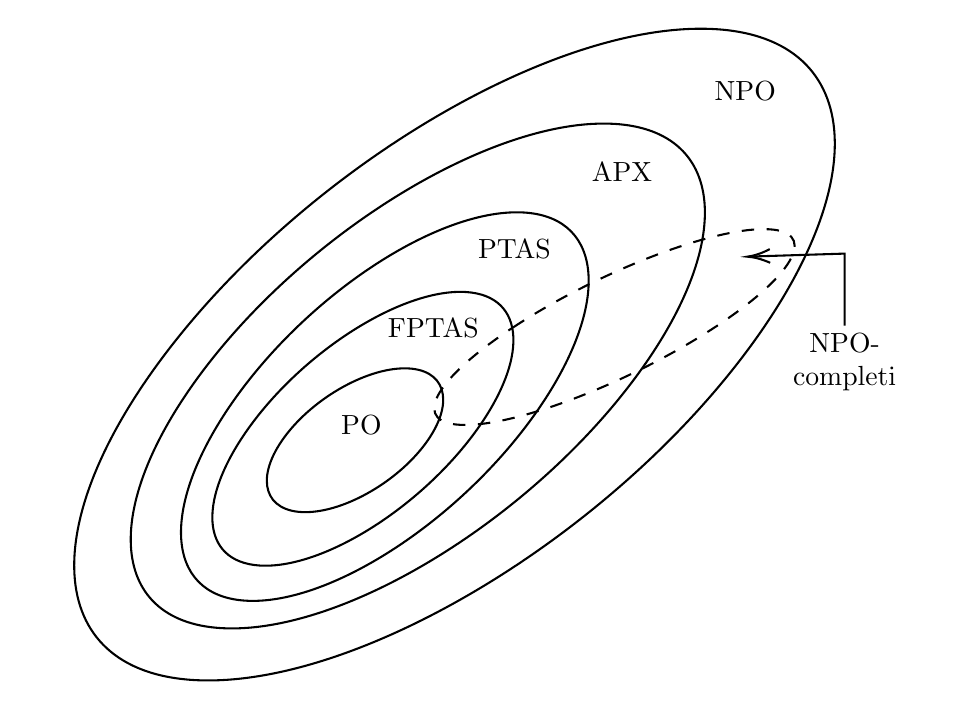
\begin{tikzpicture}[x=0.75pt,y=0.75pt,yscale=-1,xscale=1]
%uncomment if require: \path (0,477); %set diagram left start at 0, and has height of 477

%Shape: Ellipse [id:dp4588658322810296] 
\draw   (310.61,174.5) .. controls (376.13,87.79) and (491.77,17.5) .. (568.88,17.5) .. controls (645.98,17.5) and (655.37,87.79) .. (589.84,174.5) .. controls (524.31,261.21) and (408.68,331.5) .. (331.57,331.5) .. controls (254.46,331.5) and (245.08,261.21) .. (310.61,174.5) -- cycle ;
%Shape: Ellipse [id:dp4441062862246874] 
\draw   (327.15,184.82) .. controls (376.62,117.65) and (463.91,63.2) .. (522.11,63.2) .. controls (580.32,63.2) and (587.41,117.65) .. (537.94,184.82) .. controls (488.48,251.99) and (401.19,306.44) .. (342.98,306.44) .. controls (284.77,306.44) and (277.68,251.99) .. (327.15,184.82) -- cycle ;
%Shape: Ellipse [id:dp42532014972954124] 
\draw   (341.82,199.56) .. controls (376.94,147.86) and (438.92,105.95) .. (480.25,105.95) .. controls (521.58,105.95) and (526.61,147.86) .. (491.49,199.56) .. controls (456.37,251.26) and (394.39,293.17) .. (353.06,293.17) .. controls (311.73,293.17) and (306.7,251.26) .. (341.82,199.56) -- cycle ;
%Shape: Ellipse [id:dp9403889034822421] 
\draw   (350.81,210.25) .. controls (376.75,173.81) and (422.52,144.28) .. (453.04,144.28) .. controls (483.57,144.28) and (487.28,173.81) .. (461.34,210.25) .. controls (435.4,246.68) and (389.63,276.22) .. (359.11,276.22) .. controls (328.58,276.22) and (324.87,246.68) .. (350.81,210.25) -- cycle ;
%Shape: Ellipse [id:dp9056149450292196] 
\draw   (367.2,215.78) .. controls (380.43,196.64) and (406.86,181.13) .. (426.24,181.13) .. controls (445.62,181.13) and (450.6,196.64) .. (437.38,215.78) .. controls (424.15,234.91) and (397.71,250.42) .. (378.34,250.42) .. controls (358.96,250.42) and (353.97,234.91) .. (367.2,215.78) -- cycle ;
%Shape: Ellipse [id:dp18032210948172078] 
\draw  [dash pattern={on 4.5pt off 4.5pt}] (478.73,161.23) .. controls (518.48,135.18) and (572.44,114.06) .. (599.25,114.06) .. controls (626.06,114.06) and (615.57,135.18) .. (575.82,161.23) .. controls (536.07,187.29) and (482.11,208.41) .. (455.3,208.41) .. controls (428.48,208.41) and (438.98,187.29) .. (478.73,161.23) -- cycle ;
%Straight Lines [id:da10034962558485494] 
\draw    (638.18,160.5) -- (638.18,125.85) -- (593.29,127.26) ;
\draw [shift={(591.29,127.33)}, rotate = 358.2] [color={rgb, 255:red, 0; green, 0; blue, 0 }  ][line width=0.75]    (10.93,-3.29) .. controls (6.95,-1.4) and (3.31,-0.3) .. (0,0) .. controls (3.31,0.3) and (6.95,1.4) .. (10.93,3.29)   ;

% Text Node
\draw (574.07,41.64) node [anchor=north west][inner sep=0.75pt]   [align=left] {NPO};
% Text Node
\draw (514.9,80.38) node [anchor=north west][inner sep=0.75pt]   [align=left] {APX};
% Text Node
\draw (460.1,117.56) node [anchor=north west][inner sep=0.75pt]   [align=left] {PTAS};
% Text Node
\draw (416.67,155.6) node [anchor=north west][inner sep=0.75pt]   [align=left] {FPTAS};
% Text Node
\draw (394.14,202.63) node [anchor=north west][inner sep=0.75pt]   [align=left] {PO};
% Text Node
\draw (638.18,178) node   [align=left] {\begin{minipage}[lt]{51.43pt}\setlength\topsep{0pt}
\begin{center}
NPO-completi
\end{center}

\end{minipage}};


\end{tikzpicture}
\caption{Rappresentazione insiemistica delle classi di complessità.}
\label{fig:compsets}
\end{figure}



\section{Terminologia riguardante i problemi}
\subsection{Grafi}
I grafi non orientati sono $G=(V,E)$ (vertici e lati), dove 
$$
E \in {V\choose{2}}
$$
Il \textbf{grado} di un vertice $x$ $d(x)$ è il numero di lati incidenti su 
tale vertice. Il numero di vertici è $n = |V|$, mentre $m = |E|$. 
In un grafo non orientato un \textbf{cammino} di lunghezza $k$ 
$$
\pi = v_1, v_2, \cdots, v_k
$$
tale che $\forall v_{i} \in \pi :\exists \langle v_i, v_{i+1}\rangle \in E$. 
Un cammino senza ripetizioni di vertici è chiamato \textit{semplice}, altrimenti
è definito \textit{non semplice}. Un \textbf{circuito} è un cammino semplice
chiuso di lunghezza $\geq 3$. La \textbf{connessione} tra due vertici $x$ e $y$
è denotata $x \leadsto y$ e sussiste se esiste un cammino da $x$ a $y$ (e, di
conseguenza, da $y$ a $x$); questa nozione è inoltre una relazione di
equivalenza (totale), gode infatti di riflessività, transitività e simmetria.
Gli insiemi di vertici mutuamente connessi formano le \textbf{componenti
connesse} di un grafo.
